\documentclass{article}

\usepackage{booktabs}
\usepackage{tabularx}
\usepackage{adjustbox}
\usepackage{hyperref}
\usepackage{graphicx}
\usepackage{float}
\usepackage{array}
\usepackage{pdflscape}
\usepackage{longtable}

\hypersetup{
    colorlinks=true,       % false: boxed links; true: colored links
    linkcolor=red,          % color of internal links (change box color with linkbordercolor)
    citecolor=green,        % color of links to bibliography
    filecolor=magenta,      % color of file links
    urlcolor=cyan           % color of external links
}

\title{Hazard Analysis\\\progname}

\author{\authname}

\date{}

\input{../Comments}
%% Common Parts

\newcommand{\progname}{Software Engineering} % PUT YOUR PROGRAM NAME HERE
\newcommand{\authname}{Team \#2, Team Name
\\ Zihao Du 
\\ Matthew Miller
\\ Firas Elayan
\\ Abhiram Neelamraju
\\ Michael Kim} % AUTHOR NAMES                  

\usepackage{hyperref}
    \hypersetup{colorlinks=true, linkcolor=blue, citecolor=blue, filecolor=blue,
                urlcolor=blue, unicode=false}
    \urlstyle{same}
                                


\begin{document}

\maketitle
\thispagestyle{empty}

~\newpage

\pagenumbering{roman}

\begin{table}[hp]
\caption{Revision History} \label{TblRevisionHistory}
\begin{tabularx}{\textwidth}{llX}
\toprule
\textbf{Date} & \textbf{Developer(s)} & \textbf{Change}\\
\midrule
Oct 20th & All & Revision 0\\
Nov 23rd & Zihao Du & Add the new requirement IDs in the new SRS\\
Jan 7th & Zihao Du, Matthew Miller & Revision 1: Update FMEA\\
& Michael Kim, Waseef Nayeem & \\
Jan 8th & Zihao Du & Revision 1: Resolve TA feedback and peer review issues\\
Mar 5th & Zihao Du & Revision 1: Change FMEA table SR due to change of the scope in requirement documents\\
\bottomrule
\end{tabularx}
\end{table}

~\newpage

\tableofcontents

~\newpage

\pagenumbering{arabic}

\section{Symbols, Abbreviations, and Acronyms}

\renewcommand{\arraystretch}{1.2}
\begin{tabular}{l l} 
  \toprule		
  \textbf{symbol} & \textbf{description}\\
  \midrule 
  STPA & System-Theoretic Process Analysis\\
  \midrule
  SRS & Software Requirement Specification\\
  \midrule
  SQL & Structured query language\\
  \midrule
  AR & Augmented Reality\\
  \midrule
  UI & User Interface\\
  \bottomrule
\end{tabular}\\

\section{Introduction}

Based on the STPA Handbook \cite{STPA}, a system hazard is a system state or set of conditions that, together with a particular set of worst-case environmental conditions will lead to a loss. Regarding CampusConnections, our Unity-based AR social networking application, a hazard can be a condition in the game when it fails to perform the intended functions or performs unexpected behaviors when coupled with environmental conditions. This document aims to detect, analyze, assess, and eliminate or migrate potential safety and security hazards that are applicable to this application. 

\section{Scope and Purpose of Hazard Analysis}

The scope of hazard analysis is to specify all potential system hazards that may arise when using the application and discover safety and security requirements to migrate and eliminate the effects of those hazards. However, it will not include hazards related to the hardware the application is running on. It will be the choice of the user and we cannot account for all mobile devices on the market. Hazard to the society will be out of the scope as well. We will assume users intend to run the application on a normally functioning mobile device properly and efficiently. The purpose of the document is to highlight various hazards associated with the system, effects and causes of corresponding failures along with new requirements for further mitigation steps.

\section{System Boundaries and Components}
The system will be divided into the following components:
\begin{enumerate}
	\item The application's client-side feature components:
	      \begin{itemize}
		      \item Friends Component
		      \item Map and Location Component
		      \item AR Camera Component
		      \item Event/Lecture Management Component
		      \item User Profile Management Component
		      \item General application features
	      \end{itemize}
	\item ASP.NET backend server for real time messaging and location sharing sessions
	\item Firebase real-time database which will store all of user, event and lecture data
	
\quad General app features include a user login system, which will be responsible for user login and account creation, as well as notification and user accessibility management. The other features are responsible for corresponding in-game functionalities, more details can be found in the figure below. The database and user interaction are considered external to the system, the interaction between the system and external systems is described in the previous \href{https://github.com/beatlepie/4G06CapstoneProjectTeam2/blob/docs-hazard-analysis/docs/SRS/SRS.pdf}{document}.
\end{enumerate}
\begin{figure}[H]
\begin{center}
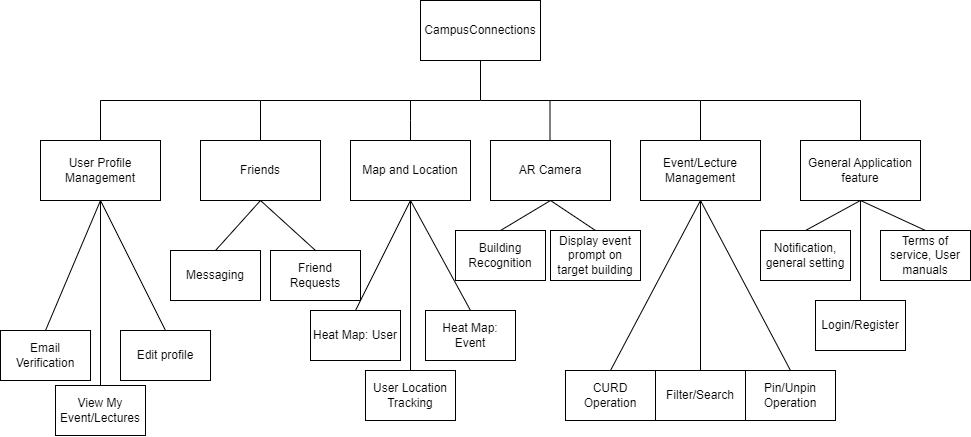
\includegraphics[scale=0.4]{components.png}
\end{center}
\caption{Client-side System Components}
\end{figure}
\section{Critical Assumptions}

\begin{itemize}
    \item Assume the administrators of the application (the developers) and the provider of lecture/event information (McMaster official website) do not intend to misuse or hack into the system (e.g. SQL injection when adding new events).
    \item Assume the user's device will have all necessary hardware components and the device OS is compatible with the application.
    \item Assume data can be transmission and storage is secure under the protection of Firebase database security rules.
    \item Assume the routes to the backend of the system will always be ready to serve requests and not blocked due to unnecessarily locked resources
    \item Assume the regular maintenance of the server and database takes very short time and does not affect users from using the application
\end{itemize}

\section{Failure Mode and Effect Analysis}
\begin{table}[H]
    \begin{adjustbox}{width=(\textwidth*6/5)}
    \centering
    

    \begin{tabular}{|p{0.20\linewidth} | p{0.20\linewidth} | p{0.20\linewidth}|  p{0.20\linewidth}|  p{0.21\linewidth}|  p{0.30\linewidth}|  p{0.08\linewidth}|p{0.07\linewidth}| }
    \hline
         \textbf{Design Functions} & \textbf{Failure Modes} & \textbf{Effects of Failure} & \textbf{Causes of Failure} &\textbf{Detection}& \textbf{Recommended Action} & \textbf{SR} & \textbf{Ref}\\
         \hline
         AR Camera      &     Building recognition fails      &      The corresponding AR objects set on the target cannot be loaded      &      a. Poor lighting conditions (e.g. in the evening)      &      a. Users cannot see any designed AR objects on the screen even if they try from different angles      &      a. Notify the user that they AR camera may have a poor performance in poor lighting condition or bad weather, give them developer's contact information for more questions      &      a. NFR-P-RF4      &      H1-1      \\
         &&&      b. Bad Weather (e.g. foggy)      &      b. Same as H1-1a      &      b. Same as H1-1a      &      b. NFR-P-RF4      &      \\
         \hline
         Backend Server     &    Server crashes      &      All services related to server (chatting, real time location map) are down      &      a. Server-side Software Error      &      a. Users cannot chat with friends or see other users on the map and error messages are found in the server logs      &      a. Let server attempt to restart once it crashes due to unknown errors      &      a. NFR-P-RF3      &      H2-1      \\
         &      Server fails to respond      &       All related services fail to render new changes      &      a. Server reaches max capacity      &      a. Error messages complaining about server over capacity are found in the log      &      a. Estimate potential user number and get an appropriate plan      &      b. NFR-P-SE1      &      H2-2      \\
         \hline
        General Application Feature      &      Internet connection is lost      &       The user is unable to send or receive data from the server     &      a. The user runs out of mobile data      &      a. The device shows there is no internet connection       &      a. Notify the user that they have lost internet connection      &      a. NFR-P-RF1      &      H3-1      \\
        &&&  b. The internet connection is poor/weak    &        b. Same as H3-1a         &  b. Same as H3-1a           &  b. NFR-P-RF1           &\\
          \hline
          Database           &    SQL injection attack         &           Personal information leakage and database information corruption           &           a. Inputs like user email and nick name are not validated           &           a. Database log shows malicious SQL statements are inserted as input           &     Limit the use of special characters for all vulnerable user input fields     &   a. NFR-P-SC5, SC6         &      H4-1            \\
                                   &&&           b. Users bypass checks in the application and access database directly            &            a. Same as H4-1a            &            a. Add protection rules from the database side      &  a. NFR-S-A1          &\\
          \hline
          Map and Location           &    Distracted walking when watching the screen         &           Users may block the traffic or even get injured because of distracted walking           &           The game-play of real time location map (User tends to walk and check the map simultaneously)           &           a. Users walk and use the application map at the same time           &     Show a warning message when using the map that tell the user to be aware of the surroundings     &   a. NFR-P-SC3          &      H5-1            \\
          \hline
    \end{tabular}
    \end{adjustbox}
    \caption{\bf FMEA Table}
    \label{tab:FMEA1}
\end{table}

\begin{table}[H]
    \begin{adjustbox}{width=(\textwidth*6/5)}
    \centering
    

    \begin{tabular}{|p{0.20\linewidth} | p{0.20\linewidth} | p{0.20\linewidth}|  p{0.20\linewidth}|  p{0.21\linewidth}|  p{0.30\linewidth}|  p{0.08\linewidth}|p{0.07\linewidth}| }
    \hline
         \textbf{Design Functions} & \textbf{Failure Modes} & \textbf{Effects of Failure} & \textbf{Causes of Failure} &\textbf{Detection}& \textbf{Recommended Action} & \textbf{SR} & \textbf{Ref}\\
         \hline
         Map and Location     &     Unintentional location sharing      &      The real time location of user outside campus is shared with other users using the map      &      a. User forgets to disconnect from real-time map session      &      a. User is marked outside of campus on the map     &      a. Check if the user location is on campus. If not, disconnect him from the map session and hide his location from other users      &      a. NFR-P-SC4      &      H5-2      \\
         \hline
         User Profile Management     &    User account is hacked      &      Sensitive personal information leakage      &      a. Week password protection rules      &      a. User report      &      a. Add password rest through email functionality      &      a. FR2-4      &      H6-1      \\
         &&&&&      b. Allow users to contact administrators to suspend target account      &      b. NFR-S-A1      & \\
         &      Malicious user creates bot accounts      &       Database and authentication system have less capacity for normal users    &      a. Lack of human verification during account creation process      &      a. lots of fake accounts are created at the same time in the authentication system log      &      a. Block guest account from connecting to the server    &      a. NFR-S-A1      &      H6-2     \\
          \hline
    \end{tabular}
    \end{adjustbox}
    \caption{\bf FMEA Table cont}
    \label{tab:FMEA2}
\end{table}

\section{Safety and Security Requirements}

The following requirements includes previous non-functional requirements in the Software Requirements Specification document that are referred in the previous section and new requirements added to handle potential hazards.

\subsection{Access Requirements}
\textbf{S-A1:} User with first level access is treated as a guest.\\
\textbf{Rationale:} User persona: a grade 12 student on a university tour.\\
\textbf{Fit Criterion:} Guest must not have access to anything beyond the login, account creation, public events, map without other users' locations and account recovery pages. \\\\
\textbf{S-A2:} User with second level access is treated as an actual user.\\
\textbf{Rationale:} User persona: a software engineer undergrad student.\\
\textbf{Fit Criterion:} User will have full access to all features except writing access to the database, which means a user cannot edit or create new lectures or events. \\\\
\textbf{S-A3:} User with third level access is treated as an administrator.\\
\textbf{Rationale:} Full access of the system should be given to administrators who works as a maintainer.\\
\textbf{Fit Criterion:} Administrator will have all the access users have and the power to add, delete and edit official events, lectures and all users profiles.\\\\

\subsection{Integrity Requirements}

\textbf{N/A}

\subsection{Privacy Requirements}
\textbf{S-P1:} The application will comply with all relevant privacy laws and guidelines.\\
\textbf{Rationale:} The application will respect the privacy of all the users.\\
\textbf{Fit Criterion:} The usage of a user’s personal information by the product abides by the Privacy Act, The Personal Information Protection and Electronic Documents Act, and Canada and Ontario’s data protection laws.\\\\
\textbf{S-P2:} Accounts that are inactive for a certain period shall be deleted after notice to prevent unnecessary data from being held.\\
\textbf{Rationale:} It prevents personal information from being stored in the database unintentionally for a long time.\\
\textbf{Fit Criterion:} Accounts that are not logged in for a semester will be cleaned from the authentication system and database.\\\\

\subsection{Audit Requirements}

\textbf{N/A}

\subsection{Immunity Requirements}

\textbf{N/A}

\subsection{New Requirements}
The following requirements in bold are the new requirements added to our SRS document.
\begin{itemize}
	\item[NFR-P-RF1.] \textbf{The product shall display an error message when there is no internet connection.}
    \begin{itemize}
        \item \textbf{Rationale:} When there is no internet connection, the user should be made aware.
        \item \textbf{Fit Criterion:} An error message stating that there is no internet connection is displayed when the product fails to connect to the internet.
    \end{itemize}
	\item[NFR-P-RF2.] \textbf{There must be a fail-safe for the product to function if the server connection takes too long or fails.}
    \begin{itemize}
        \item \textbf{Rationale:} This will allow the product to function to some degree even during high traffic or bad server connection situations.
        \item \textbf{Fit Criterion:} The product must be able to provide rudimentary functionalities without connecting to the internet or server.
    \end{itemize}
	\item[NFR-P-RF3.] \textbf{The server shall attempt to restart when it crashes.}
    \begin{itemize}
        \item \textbf{Rationale:} This requirement enhances the robustness of the backend server and prevents it from going down for a long time because of some intermittent minor errors.
        \item \textbf{Fit Criterion:} The server should try to restart after it crashes due to unknown errors.
    \end{itemize}
	\item[NFR-P-RF4.] \textbf{AR Camera should have a notification available in the UI telling users possible reasons the target is not recognized.}
    \begin{itemize}
        \item \textbf{Rationale:} The user should get a notification telling them that the AR camera may have a bad performance in some cases, and they should be able to report that to the developer if they want the problem to be solved.
        \item \textbf{Fit Criterion:} The product should show the user a list of possible reasons that the camera does not work and the contact information of maintainers once they have trouble using the AR camera and click the help button.
    \end{itemize}
    \item[NFR-P-SC3.] \textbf{The product shall display a message upon map startup warning the user to be aware of their surroundings.}
    \begin{itemize}
        \item \textbf{Rationale:} The game-play of real-time location map may lead to distracted walking, therefore we need to warn the user for their safety.
        \item \textbf{Fit Criterion:} A message telling the user to be aware of their surroundings is displayed upon map startup.
    \end{itemize}
    \item[NFR-P-SC4.] \textbf{The product shall hide user's location if the user leaves campus.}
    \begin{itemize}
        \item \textbf{Rationale:} Users may stay connected and share their location even when they leave the campus. To prevent personal information leakage, we need to hide that information and disconnect the user.
        \item \textbf{Fit Criterion:} A user's information shall not be shared once he or she leaves campus.
    \end{itemize}
    \item[NFR-P-SC5.] \textbf{The product shall prevent the user from entering special characters in all text input fields.}
    \begin{itemize}
        \item \textbf{Rationale:} When creating accounts, users can perform SQL injection attacks by inputting some SQL statements.
        \item \textbf{Fit Criterion:} Any text input with special characters will give the user an error.
    \end{itemize}
    \item[NFR-P-SC6.] \textbf{The product shall validate the email format when creating an account.}
    \begin{itemize}
        \item \textbf{Rationale:} When creating accounts, users can perform SQL injection attacks by inputting some SQL statements.
        \item \textbf{Fit Criterion:} An input in the email field that's not in the format of an email will give the user an error when creating a new account.
    \end{itemize}
\end{itemize}

\section{Roadmap}

The hazard analysis has identified lots of safety and security requirements, but due to time constraints,  not all of the requirements can be fulfilled. Our team thinks the following requirements have higher priority and will implement them for the capstone:
\begin{itemize}
    \item AR Camera should have a notification available in the UI telling users possible reasons the target is not recognized.
    \item The server shall attempt to restart when it crashes.
    \item There must be a fail-safe for the product to function if server or internet connection takes too long or fails.
    \item The product shall display a message upon map startup warning the user to be aware of their surroundings.
    \item The product shall hide user location if the user leaves campus.
    \item The product shall prevent user entering special characters in all text input field.
    \item The product shall validate email format when creating an account.
\end{itemize}

\noindent
Requirements to be implemented after capstone:
\begin{itemize}
    \item The product shall display an error message when there is no internet connection.
\end{itemize}

\newpage

\begin{thebibliography}{9}
  \bibitem{STPA} Nancy G. Leveson and John P. Thomas. \emph{STPA Handbook.} March 2018.
\end{thebibliography}

\end{document}